\documentclass[a4paper]{article}
\usepackage{geometry}
% Set the margins
\geometry{
    a4paper,
    total={170mm,257mm},
    left=20mm
}

\usepackage{csvsimple}
\usepackage{subcaption}
\usepackage{listings}
\usepackage{xcolor}

\definecolor{codegreen}{rgb}{0,0.6,0}
\definecolor{codegray}{rgb}{0.5,0.5,0.5}
\definecolor{codepurple}{rgb}{0.58,0,0.82}
\definecolor{backcolour}{rgb}{0.95,0.95,0.92}

\lstdefinestyle{mystyle}{
    backgroundcolor=\color{backcolour},   
    commentstyle=\color{codegreen},
    keywordstyle=\color{magenta},
    numberstyle=\tiny\color{codegray},
    stringstyle=\color{codepurple},
    basicstyle=\ttfamily\footnotesize,
    breakatwhitespace=false,         
    breaklines=true,                 
    captionpos=b,                    
    keepspaces=true,                 
    numbers=left,                    
    numbersep=5pt,                  
    showspaces=false,                
    showstringspaces=false,
    showtabs=false,                  
    tabsize=2
}
\lstset{style=mystyle}
\usepackage{subcaption}
\usepackage{graphicx}
\graphicspath{{./Images/}}

\title{COMP24112 Lab Report}
\author{Licheng Chen}

\begin{document}
\maketitle

\section{Linear Classification via Gradient Descent}

\subsection{Derivation of the training objection function}

$$O = C \sum^N_{i=1}\max\left(0, 1 - y_i \left(\mathbf{w}^T\mathbf{x}_i + w_0\right)\right) + \frac{1}{2}\mathbf{w}^T\mathbf{w}. $$


\newpage
\subsection{Model Training and Testing}
\begin{figure}[htbp]
    \centering
    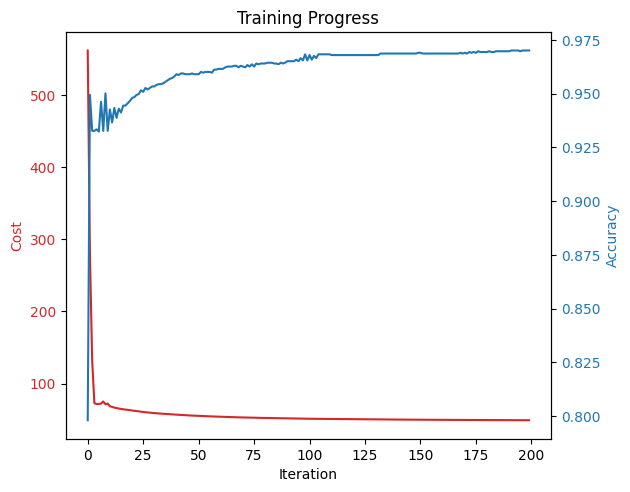
\includegraphics[width=0.5\linewidth]{1.1.png}
    \caption{\centering Graph of the cost and accuracy of training over iterations}
\end{figure}

The model produced by the run shown above had an accuracy of 0.9677 and a F1 score of 0.7241 when run on the test data.
While initially very high, the cost of each iteration reduced dramatically, quickly falling below 100, before stabilising.
In the first 25 iterations the accuracy was rather spiky, suggesting that the models parameters are oscillating around the optimal values, before stabilising in the later iterations.
This is probably caused by the fact that I chose to initialise my weights as zeros instead of randomising them. As this behaviour was not observed when I used randomised weights.

\subsection{Learning Rate Analysis}

\begin{figure}[htbp]
    \centering
    \begin{subfigure}[b]{0.49\linewidth}
        \centering
        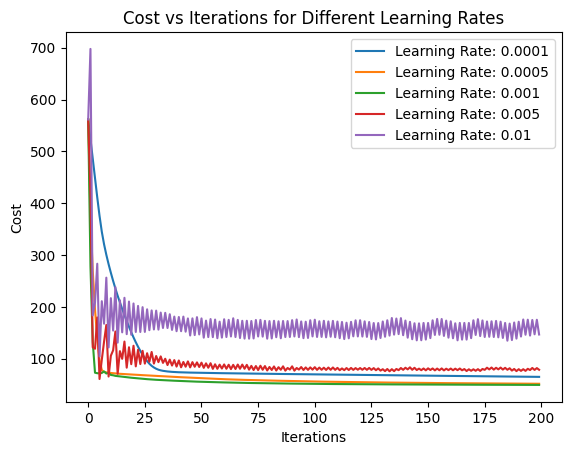
\includegraphics[width=\linewidth]{1.21.png}
        \caption{\centering Costs per iteration for various learning rates.}
    \end{subfigure}
    \hfill
    \begin{subfigure}[b]{0.49\linewidth}
        \centering
        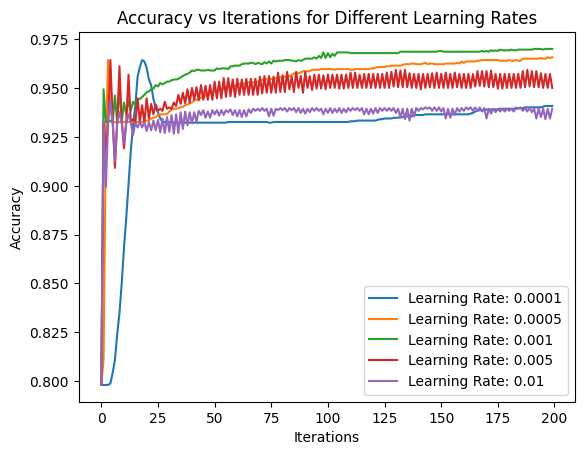
\includegraphics[width=\linewidth]{1.22.png}
        \caption{\centering Accuracy per iteration for various learning rates.}
    \end{subfigure}
    \caption{\centering Comparison of costs and accuracy per iteration for various learning rates.}
\end{figure}


\newpage
\section{Air Quality Analysis by Neural Network}
\subsection{Model Selection}


\newpage
\subsection{Training Algorithm Comparison: SGD and ADAM}

\newpage
\section{Building A Robust MLP Regressor}


\end{document}